\documentclass[a4paper,12pt]{article}
\usepackage[top = 2.5cm, bottom = 2.5cm, left = 2.5cm, right = 2.5cm]{geometry}
\usepackage[T1]{fontenc}
\usepackage[utf8]{inputenc}
\usepackage{multirow} 
\usepackage{booktabs} 
\usepackage{graphicx}
\usepackage[spanish]{babel}
\usepackage{setspace}
\setlength{\parindent}{0in}
\usepackage{float}
\usepackage{fancyhdr}
\usepackage{amsmath}
\usepackage{amssymb}
\usepackage{amsthm}
\usepackage{natbib}
\usepackage{graphicx}
\usepackage{subcaption}
\usepackage{booktabs}
\usepackage{etoolbox}
\usepackage{apalike}
\usepackage{minibox}
\usepackage{hyperref}
\usepackage{xcolor}
\usepackage{tcolorbox}
\AtBeginEnvironment{align}{\setcounter{equation}{0}}
\newenvironment{solution}
  {\renewcommand\qedsymbol{$\square$}\begin{proof}[\textcolor{blue}{Solución}]}
  {\end{proof}}

\pagestyle{fancy}

\fancyhf{}

\lhead{\footnotesize Ecuaciones Diferenciales 2}
\rhead{\footnotesize  Rudik Roberto Rompich}
\cfoot{\footnotesize \thepage}

\begin{document}
    \thispagestyle{empty} 
    \begin{tabular}{p{15.5cm}}
    \begin{tabbing}
    \textbf{Universidad del Valle de Guatemala} \\
    Departamento de Matemática\\
    Licenciatura en Matemática Aplicada\\\\
   \textbf{Estudiante:} Rudik Roberto Rompich\\
   \textbf{E-mail:} \textcolor{blue}{ \href{mailto:rom19857@uvg.edu.gt}{rom19857@uvg.edu.gt}}\\
   \textbf{Carné:} 19857
    \end{tabbing}
    \begin{center}
        MM2030 - Ecuaciones Diferenciales 2 - Catedrático: Dorval Carías\\
        \today
    \end{center}\\
    \hline
    \\
    \end{tabular} 
    \vspace*{0.3cm} 
    \begin{center} 
    {\Large \bf Cheatsheet - Ecuaciones Diferenciales
} 
        \vspace{2mm}
    \end{center}
    \vspace{0.4cm}
    %---------------------------
%\begin{tcolorbox}[colback=gray!15,colframe=black!1!black,title=A nice heading]
%\end{tcolorbox}

%\fbox{lol}
%---------------------------
\begin{center}
    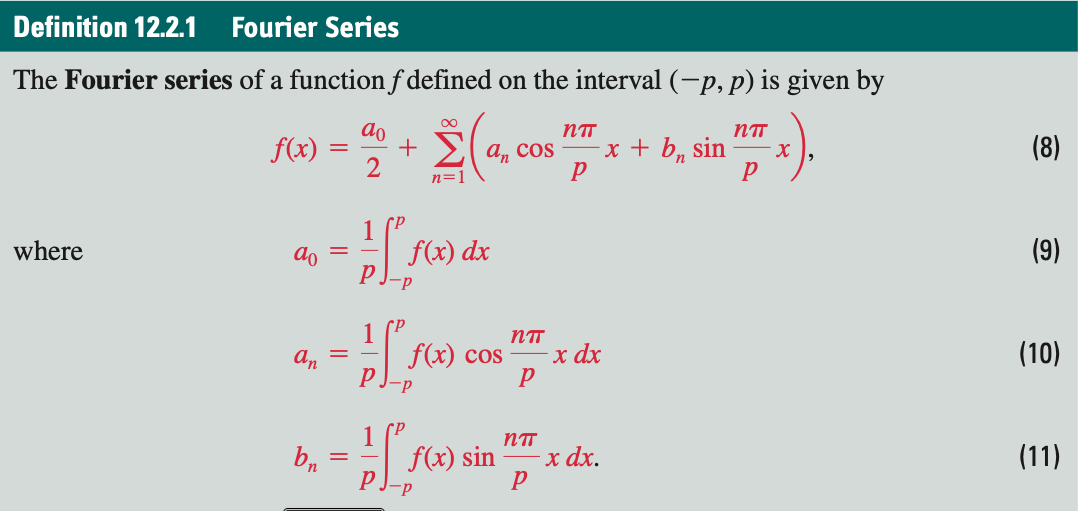
\includegraphics[scale=0.35]{images/Fourier.png}
\end{center}
\begin{center}
    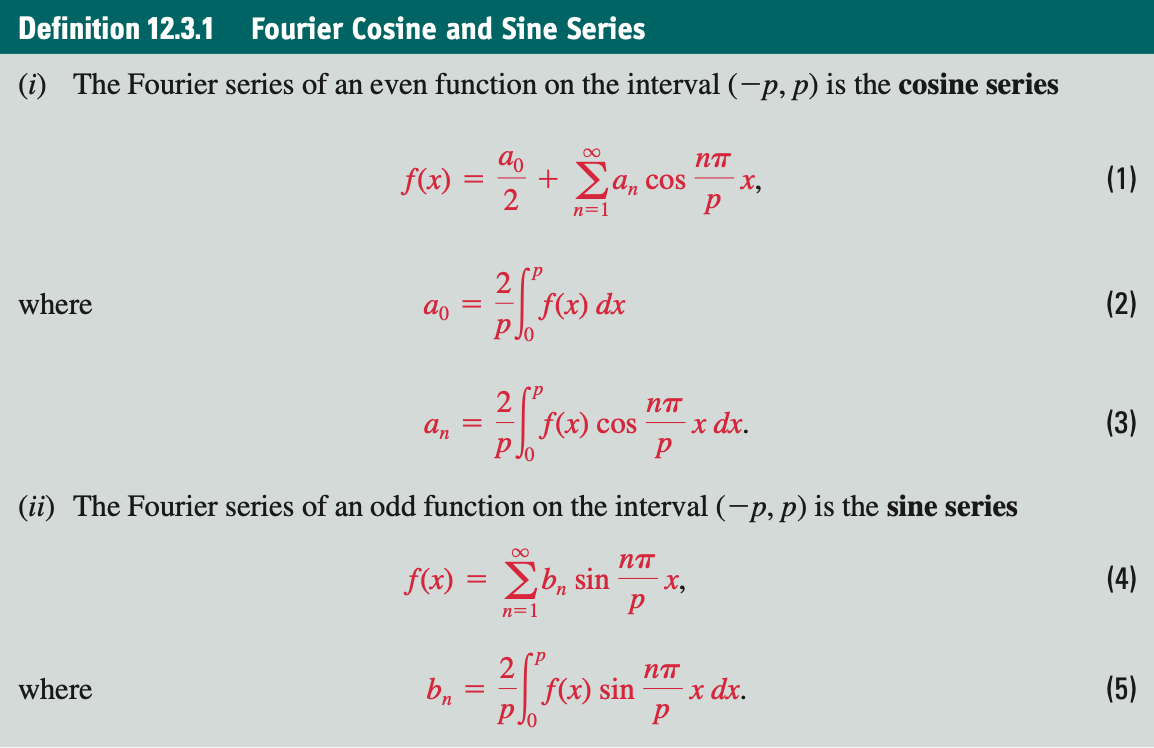
\includegraphics[scale=0.3]{images/Sin-Cosin.png}
\end{center}
\begin{center}
    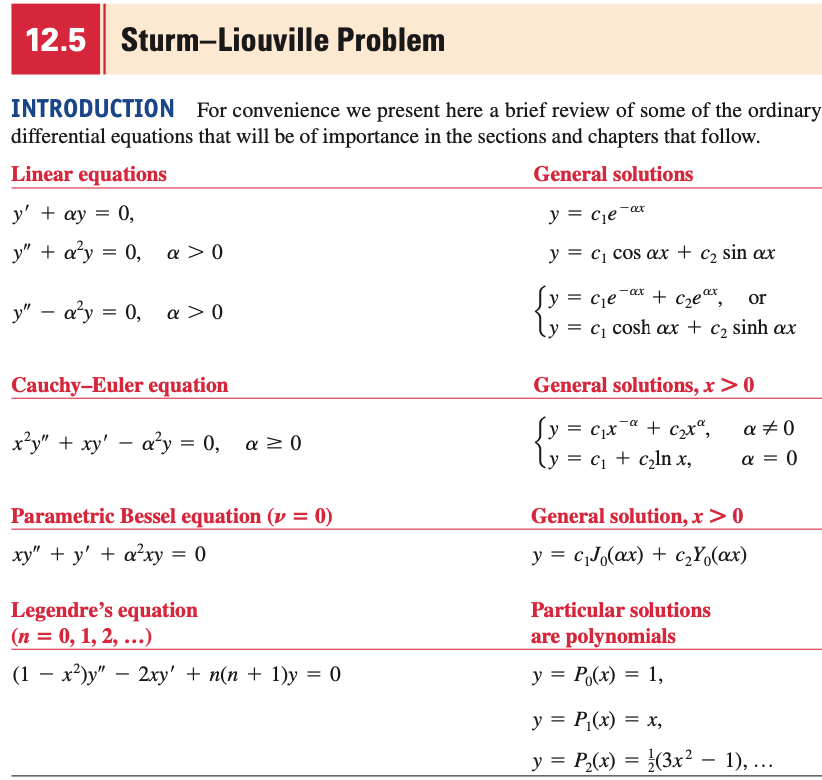
\includegraphics[scale=0.5]{images/Ordinary.png}
\end{center}
\begin{tcolorbox}[colback=gray!15,colframe=red!1!red,title=Función Gamma]
La función Gamma de Euler es: 
\begin{gather*}
    \Gamma(x)=\int_0^\infty t^{x-1}e^{-t}dt 
\end{gather*}
la convergencia de la integral requiere que $x>0$.\newline

\textbf{Relación de recurrencia}: 
\begin{gather*}
    \Gamma(x+1)= x\Gamma(x) 
\end{gather*}\newline 
\textbf{Función factorial generalizada}. Si $n$ es un número entero positivo, entonces: 
\begin{gather*}
    \Gamma(n+1)= n!
\end{gather*}
Caso especial: 
\begin{gather*}
    r\left(\frac{1}{2}\right) = \sqrt{\pi}
\end{gather*}
\end{tcolorbox}
%------------------------------------------
\begin{tcolorbox}[colback=gray!15,colframe=red!1!red,title=Ecuaciones de Bessel]
\textbf{Ecuación de Bessel}
\begin{center}
    \fbox{$x^2y''+xy'+(x^2-v^2)y=0,\quad v\geq 0$}
\end{center}
\textbf{Soluciones}
\begin{enumerate}
    \item Si $m_1-m_2=v-(-v)=2v\ \not\in \mathbb{Z}^+$. Entonces: 
    \begin{enumerate}
        \item $J_v(x)=\sum_{n=0}^{\infty}\frac{(-1)^n}{n!\Gamma(1+v+n)}\left(\frac{x}{2}\right)^{2n+v}$
        \item $J_{-v}(x)=\sum_{n=0}^{\infty}\frac{(-1)^n}{n!\Gamma(1-v+n)}\left(\frac{x}{2}\right)^{2n-v}$
    \end{enumerate}
    \begin{center}
        \fbox{$y=AJ_v(x)+BJ_{-v}(x)\quad v\neq \text{entero}$}
    \end{center}
   \item Si $m_1-m_2=v-(-v)=2v\ \in \mathbb{Z}^+$. Entonces: 
    \begin{enumerate}
        \item $J_v(x)=\sum_{n=0}^{\infty}\frac{(-1)^n}{n!\Gamma(1+v+n)}\left(\frac{x}{2}\right)^{2n+v}$
        \item $Y_v(x)= \frac{\cos v\pi J_v(x)-Y_v(x)}{\sin v\pi}$
    \end{enumerate}
    \begin{center}
        \fbox{$y=AJ_v(x)+BY_{v}(x)$}
    \end{center}
\end{enumerate}

\end{tcolorbox}

\begin{tcolorbox}[colback=gray!15,colframe=red!1!red,title=Ecuaciones de Legendre]
\textbf{Ecuación de Legendre}
\begin{center}
    \fbox{$(1-x^2)y''-2xy'+n(n+1)y=0$}
\end{center}
\textbf{Soluciones:}
\begin{enumerate}
    \item $y=P_0(x)=1$
    \item $y=P_1(x)=x$
    \item $y=P_2(x)=\frac{1}{2}(3x^2-1)$
    \item $y=P_3(x)=\frac{1}{2}(5x^3-3x)$
    \item $y=P_4(x)=\frac{1}{8}(35x^4-30x^2+3)$
    \item $y=P_5(x)=\frac{1}{8}(63x^5-70x^3+15x)$
\end{enumerate}
\textbf{Cálculo:}\newline 
Recurrencia
\begin{center}
    \fbox{$(k+1)P_{k+1}(x)-(2k+1)xP_k(x)+kP_{k-1}(x)=0$}
\end{center}
Fórmula de Rodrigues
\begin{center}
    \fbox{$P_n(x)=\frac{1}{2^nn!}\frac{d^n}{dx^n}(x^2-1)^n, \quad n\in \mathbb{N}$}
\end{center}
\end{tcolorbox}

\begin{center}
    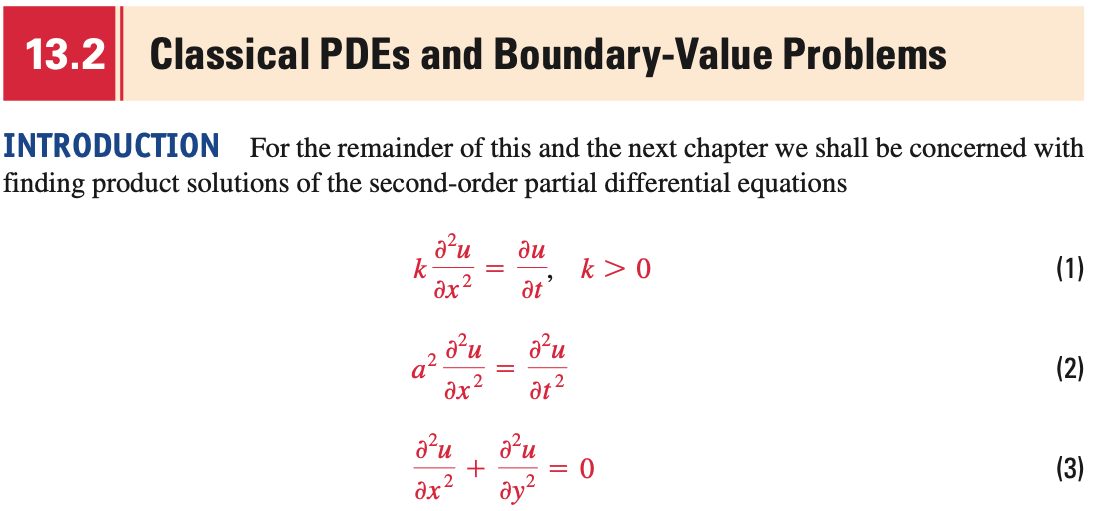
\includegraphics[scale=0.4]{images/13,2.png}
\end{center}


%---------------------------
%\bibliographystyle{apalike}
%\bibliography{sample.bib}

\end{document}